\documentclass[colorlinks=true,pdfstartview=FitV,linkcolor=blue,
            citecolor=red,urlcolor=magenta]{ligodoc}

\usepackage{graphicx}
\usepackage{amssymb}
\usepackage{amsmath}
\usepackage{longtable}
\usepackage{rotating}
\usepackage[usenames,dvipsnames]{color}
\usepackage{fancyhdr}
\usepackage{subfigure}
\usepackage{hyperref}
\usepackage{array}
\usepackage{subcaption}


\usepackage{appendix}

\title{Methods of Improving Optical Contacting

Second Interim Report}

\author{Jennifer Hritz}

\begin{document}

\section{Work completed}

Where I left off in first interim report: after spending a few weeks designing bond quality tests, I had finalize the design for heating the glass slides and was preparing to start actual bonding. Since then, I have been experimenting with the different bonding methods, exploring what factors into creating a strong bond between glass slides. For a theoretical discussion on the different bonding methods, see Appendix TBD.

\subsection{Hot plate}

I started by first determining the heating properties of the hot plate using a thermocouple. Since the bonded samples will need to be heated evenly at a precise temperature, I measured the maximum temperature at each dial setting and the temperature at different locations on the hot plate, as seen in Figure \ref{fig:hotplate_heat_test_setup}.

\begin{figure}[htbp]
\begin{center}
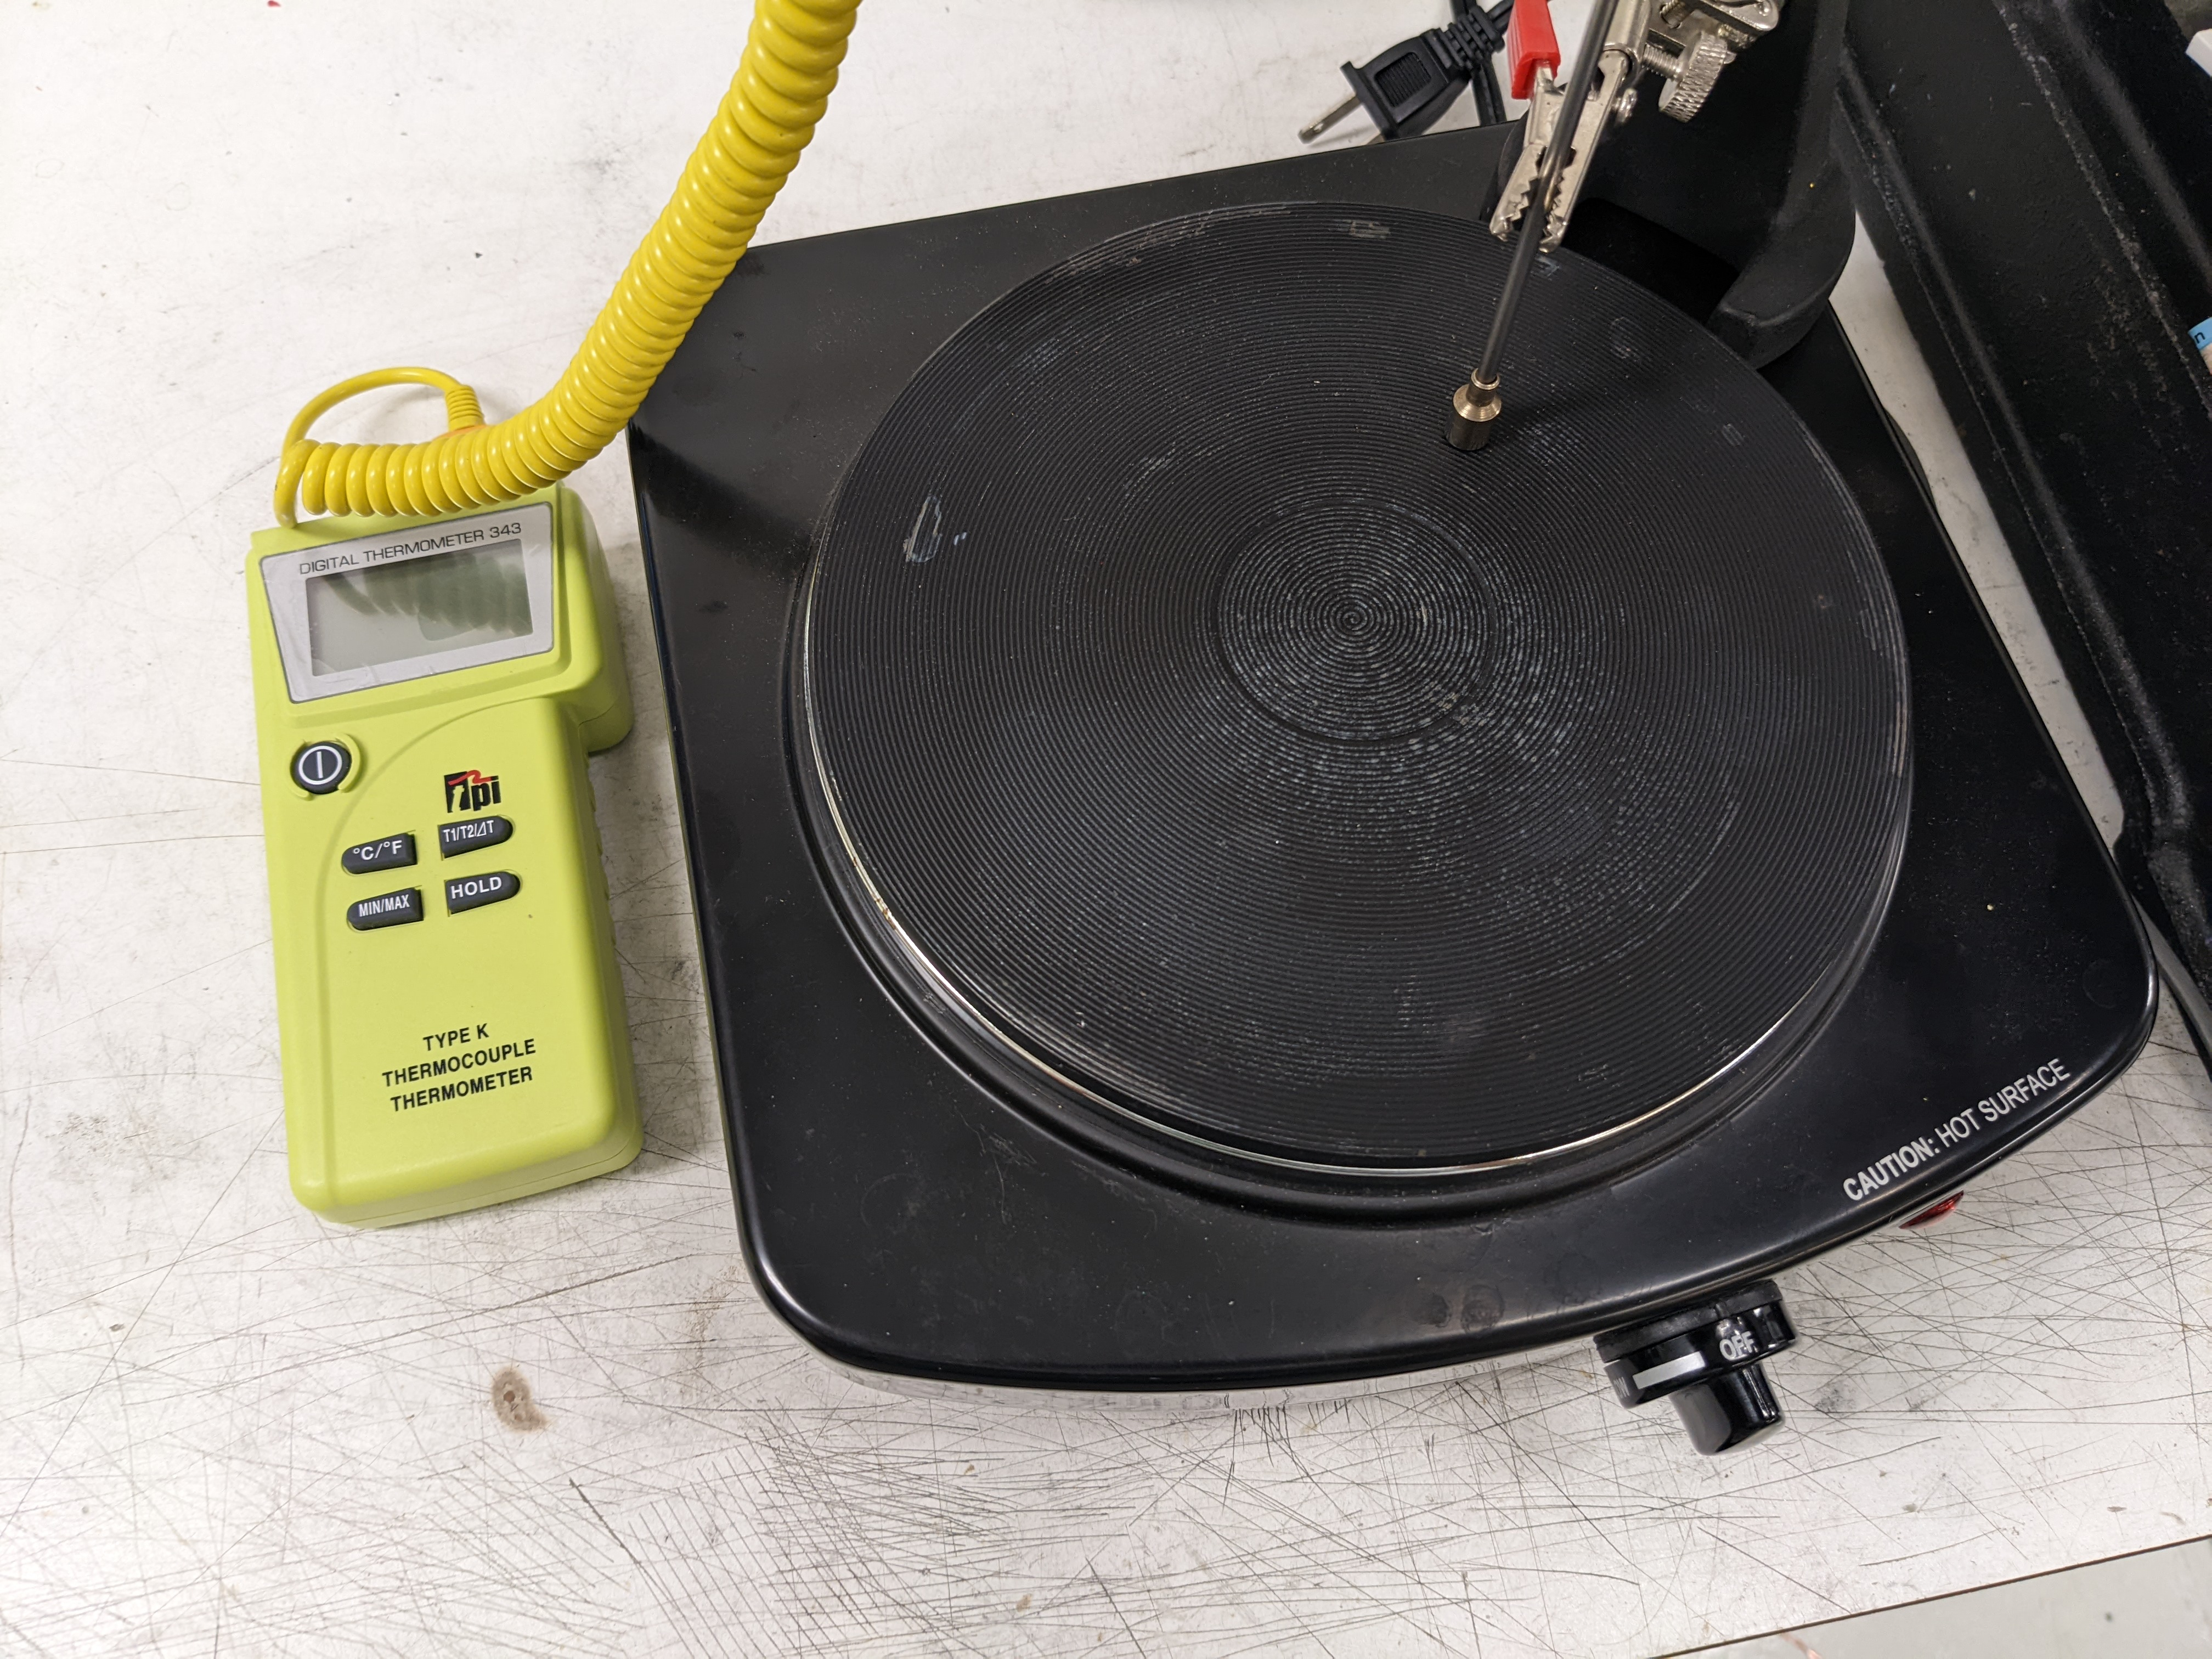
\includegraphics[width=6in]{graphics/hotplate_heat_test_setup_PXL_20220708_230032062.jpg}
\caption{The Type K thermocouple was attached to the Digital Thermometer 343, and the measuring tip of the thermocouple was mounted parallel against the Oster hot plate. Per the thermometer manual, the tip must be held in place for at least 30 seconds to get an accurate reading.}
\label{fig:hotplate_heat_test_setup}
\end{center}
\end{figure}

To measure the maximum temperature at each setting, I turned the dial and waited until the temperature of the thermometer stayed constant for over 1 minute. I then recorded the exact temperature and the rough time it took to stabilize (Figure \ref{fig:hotplate_heat_test_setup}). Once the data was collected, I turned the dial to the next setting, performing this for the low, medium, and high settings.

\begin{figure}[htbp]
\begin{center}
  \begin{tabular}{ | l | c | c | c | c | c | }
    \hline
    Setting & Off & Low & Medium & High & Off (Again) \\ \hline
    Max. temp. (°C) & 26.2 & 51.3 & 185.0 & 263.5 &N/A \\ \hline
    Time to temp. (min)  & N/A & 5.5 & 7.0 & 6.0 & $\sim$ 3 hours \\
    \hline
  \end{tabular}
\end{center}
\caption{The results of finding the maximum temperature at each hotplate knob setting. Note that "Time to temp." is the time from when the dial was switch up to when the temperature stabilized. The times are meant to only be rough estimates since I was multitasking during the experiment and not watching the plate the entire time. "Off (Again)" is the rough amount of time it took for the plate to completely cool down.}
\label{fig:hotplate_max_heat_data}
\end{figure}

Once the temperature at the high setting stabilized, I moved the thermocouple to different parts of the hot plate, being careful to keep the measuring tip parallel and to hold it steady for over 30 seconds. As seen in \ref{fig:even_heating_test_results}, the top right corner is slightly cooler and the hot plate is the hottest in a ring at about half the radius, likely where the heating coil sets.

\begin{figure}[htbp]
\begin{center}
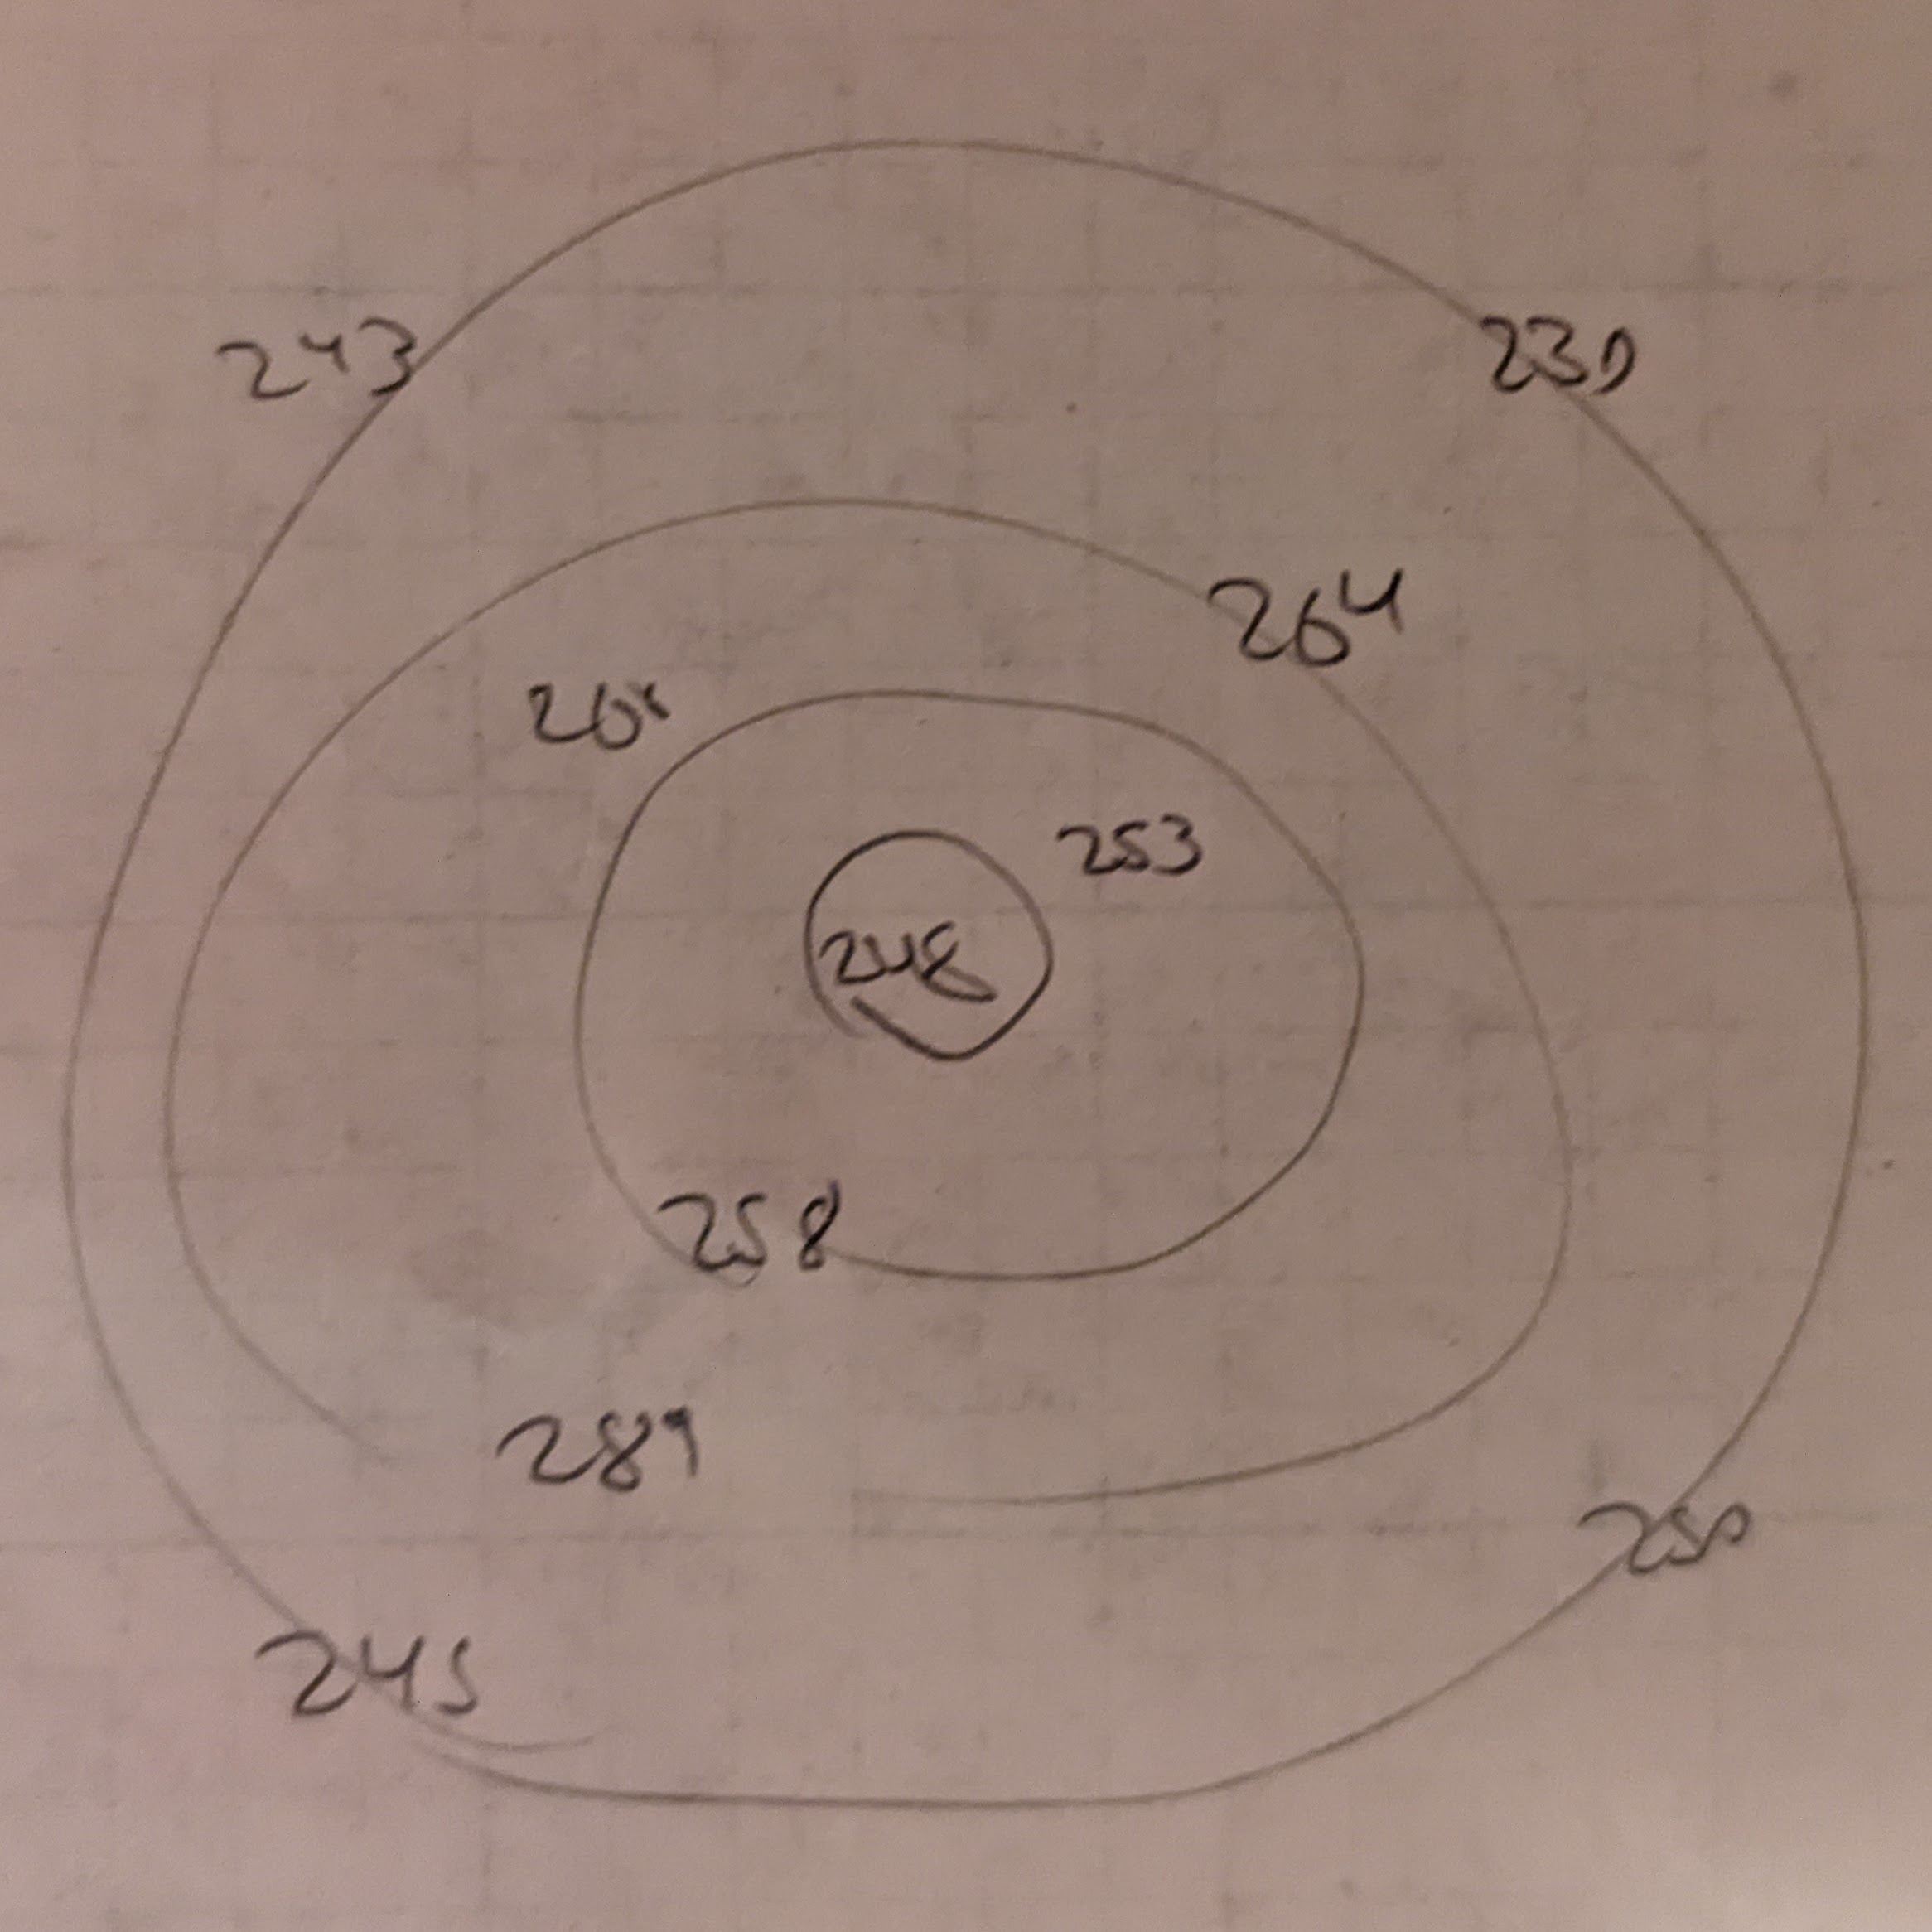
\includegraphics[width=6in]{graphics/even_heating_test_results_PXL_20220729_050013935.jpg}
\caption{The temperature (°C) at different points on the hot plate. The bottom of the circle is the side of the hot plate with the nob. It was a coincidence that the  thermocouple was set up in the cool corner during the maximum temperature test.}
\label{fig:even_heating_test_results}
\end{center}
\end{figure}

This was meant to be a rough baseline test. Once I find a way to control the temperature beyond the three settings, I will need to repeat it with a newer, more accurate multimeter.

\subsection{Bonding}

Before working with delicate silicon wafers, I started with attempting to bond 25 mm x 75 mm x 1.1 mm borosilicate glass microscope slides manufactured by Globe. I tried a variety of methods to get a feel for what worked and what did not.

I began by gently cleaning the slides with Kimwipes then carefully laying one slide on top of the other. When the top slide was lifted up, the bottom slide would hang on for at most a couple seconds before gravity overcame the bond (Figure \ref{fig:kimwipe_bond}). Pressure, with my fingers or a large brass rectangle and heat, on any of the settings, as well as the two combined did not improve the bond.

\begin{figure}
\begin{center}
\begin{subfigure}
  \centering
  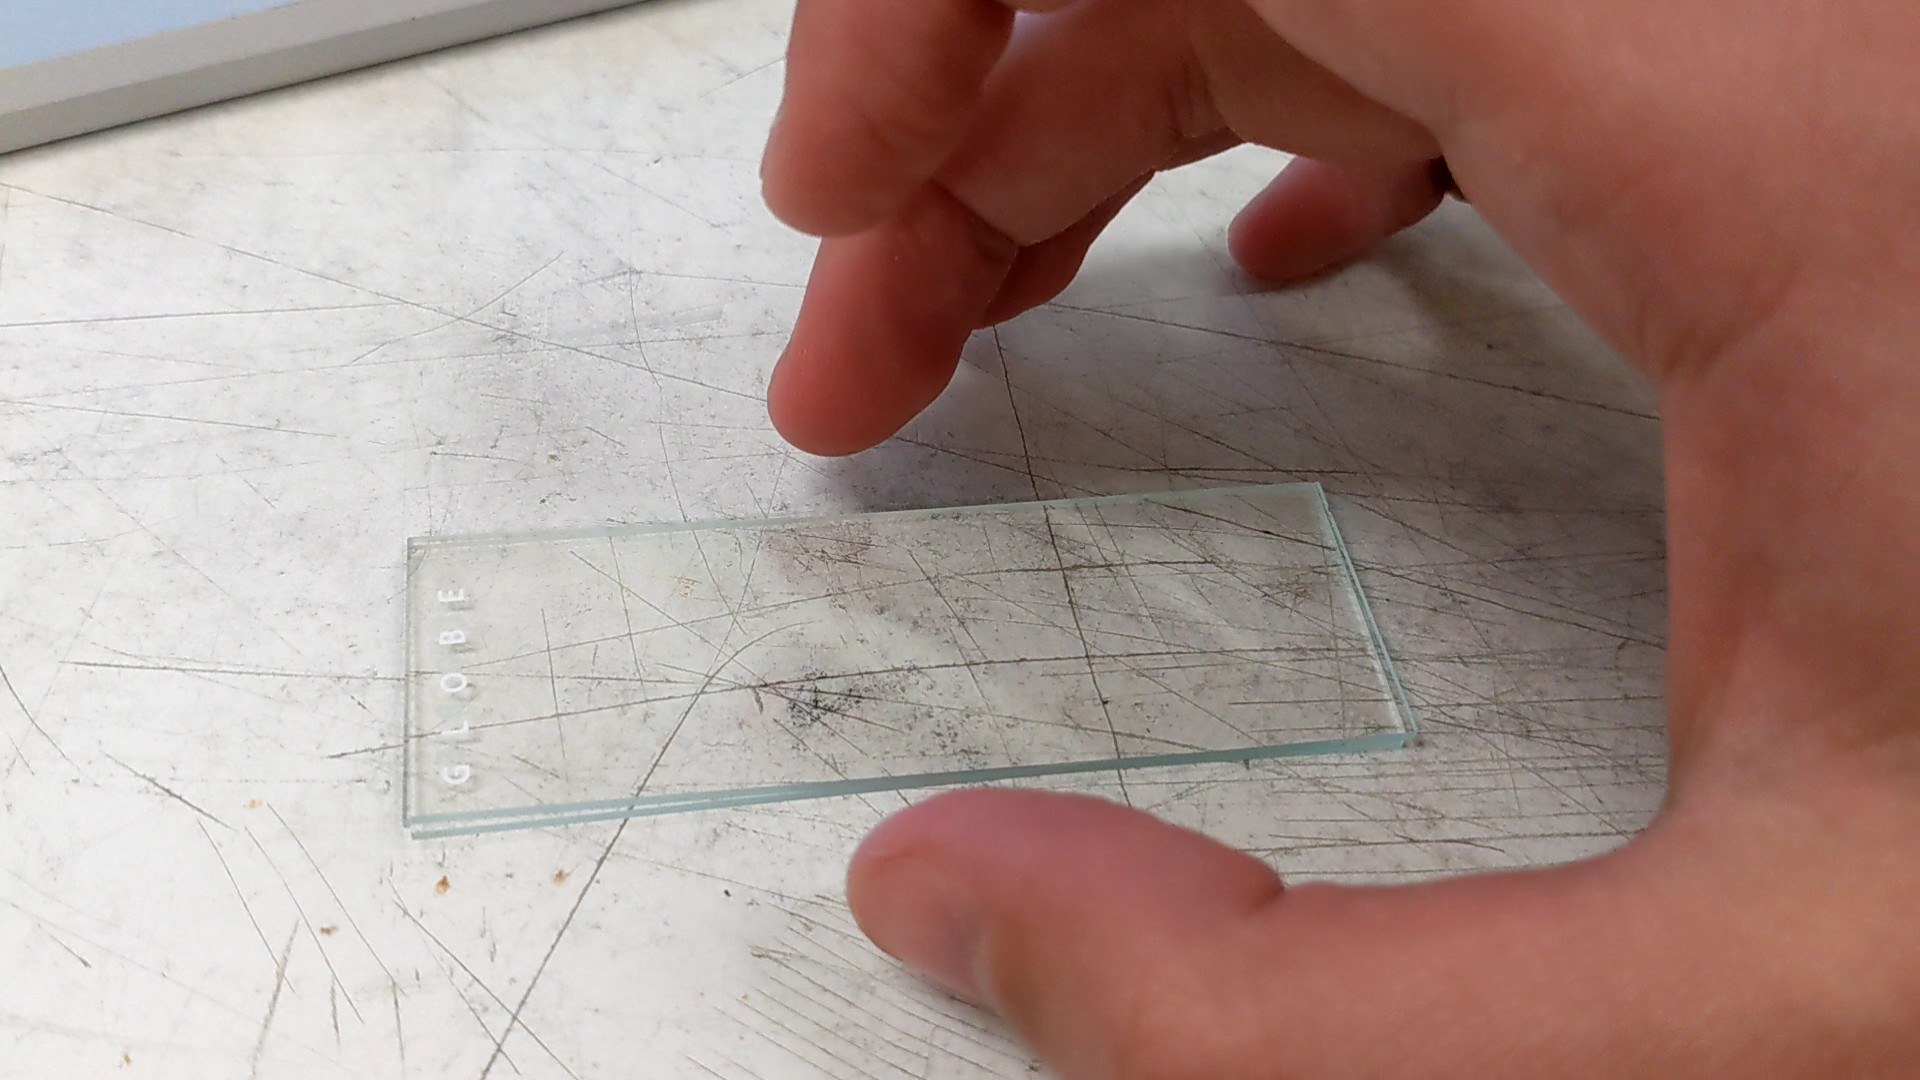
\includegraphics[width=4in]{graphics/kimwipe_before_PXL_20220712_003150428_exported_33.jpg}
  \caption{After bonding attempt.}
  \label{fig:kimwipe_bond_sfig1}
\end{subfigure}
\begin{subfigure}
  \centering
  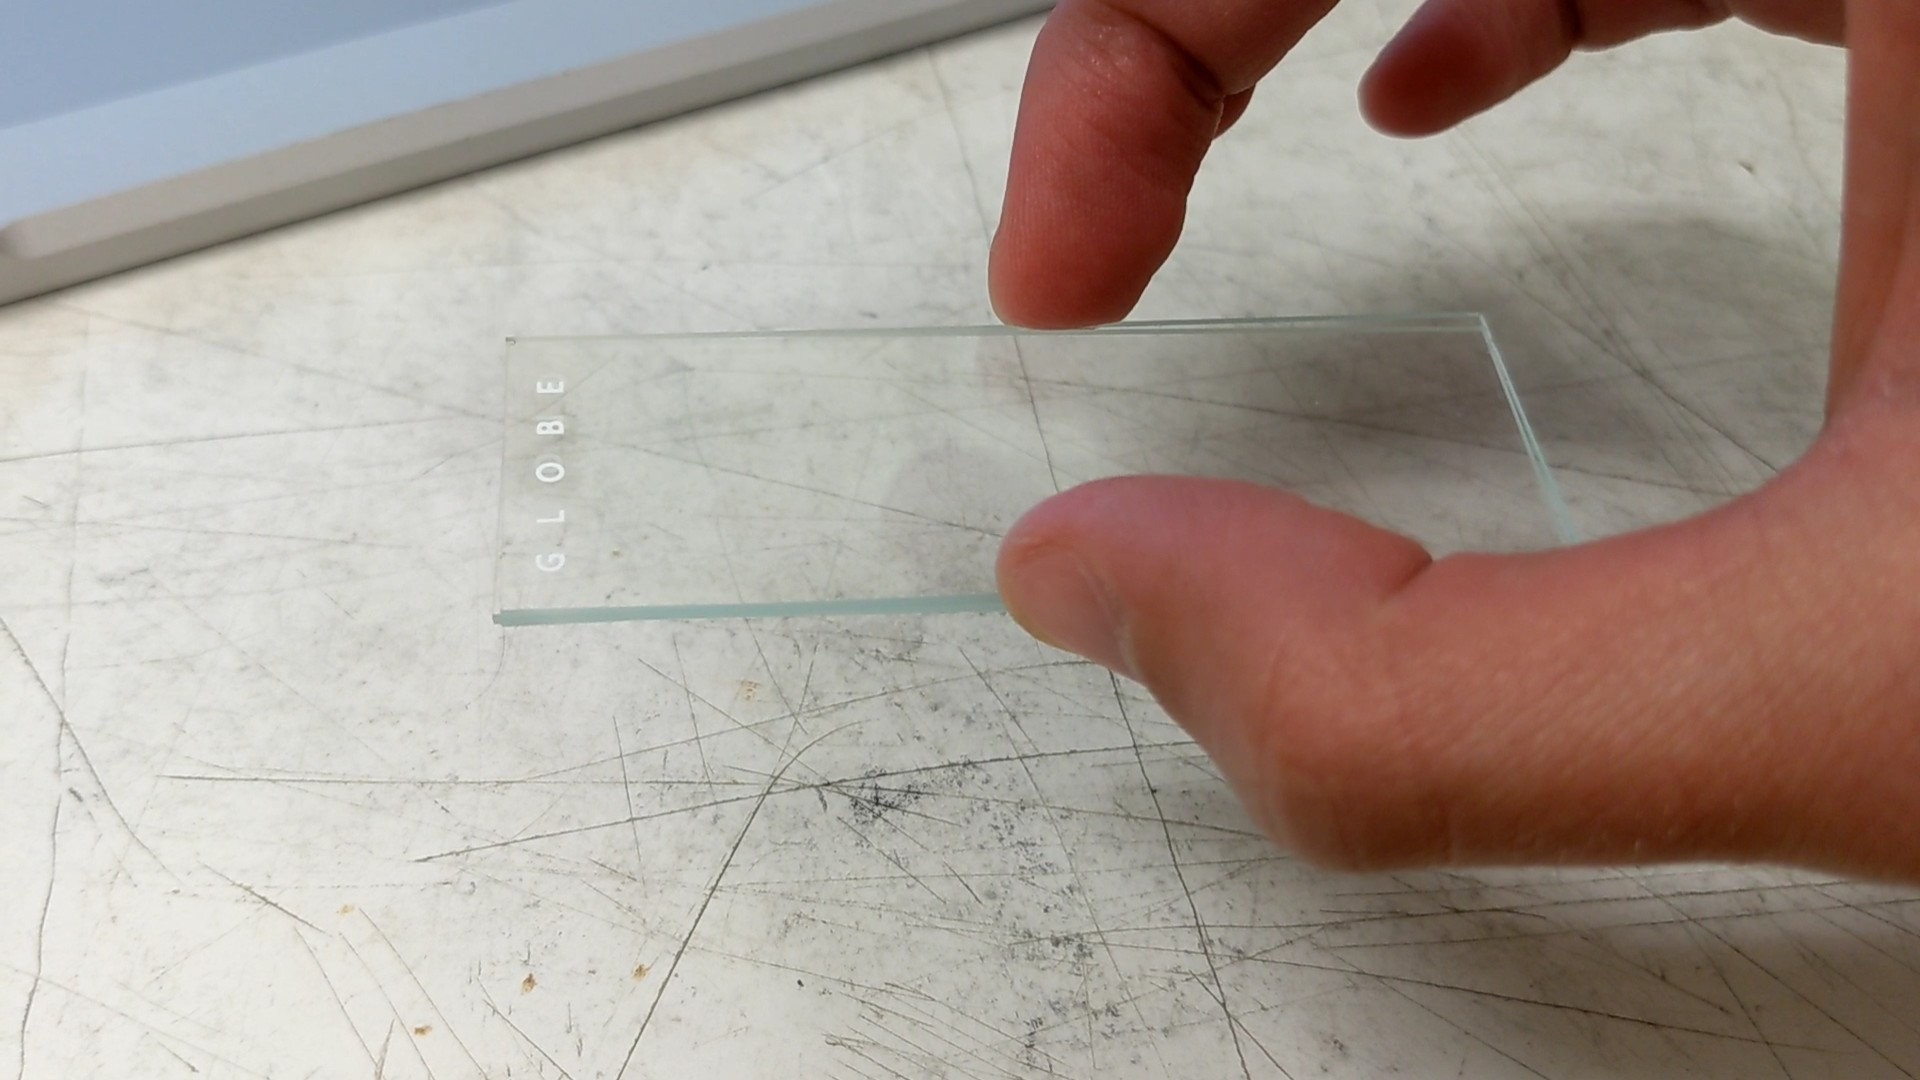
\includegraphics[width=4in]{graphics/kimwipe_during_PXL_20220712_003150428_exported_3069.jpg}
  \caption{The bond briefly holding.}
  \label{fig:kimwipe_bond_sfig2}
\end{subfigure}
\begin{subfigure}
  \centering
  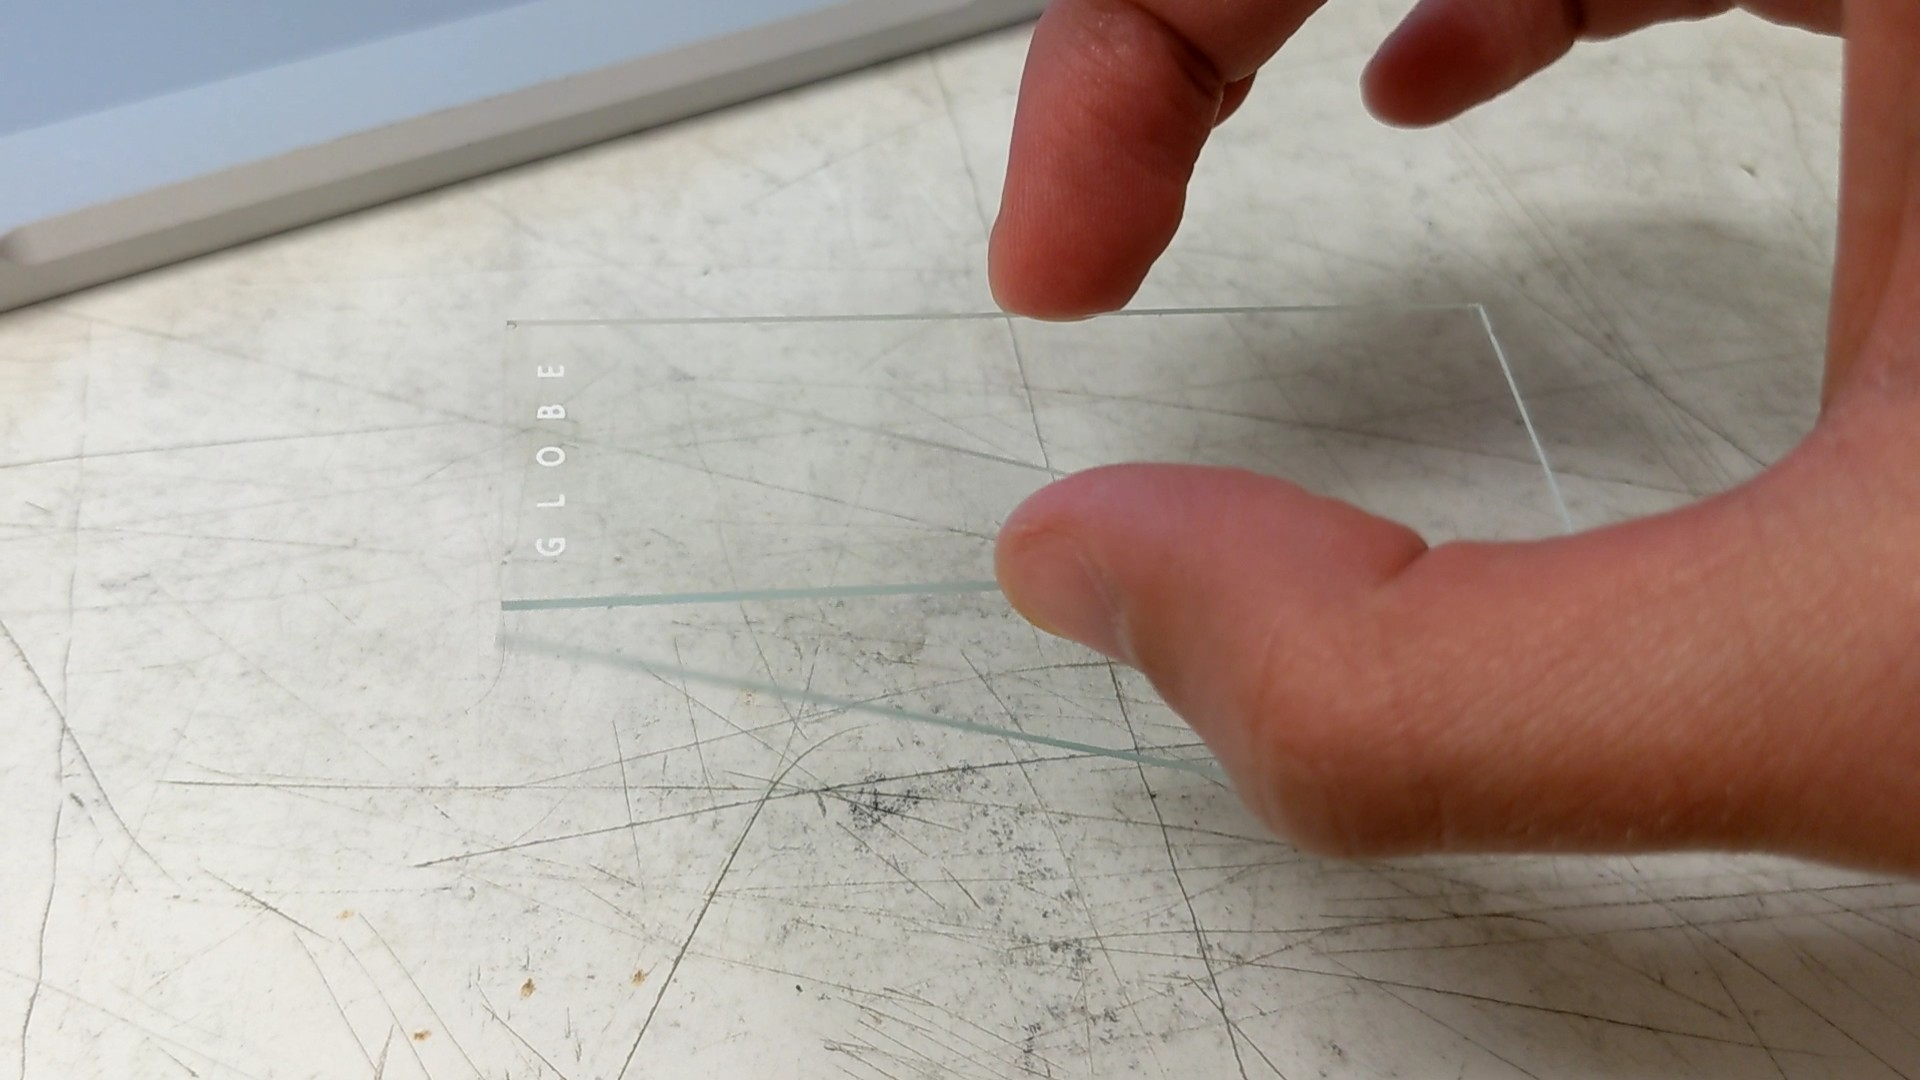
\includegraphics[width=4in]{graphics/kimwipe_after_PXL_20220712_003150428_exported_3069.jpg}
  \caption{Failure of the bond.}
  \label{fig:kimwipe_bond_sfig3}
\end{subfigure}
\caption{These demonstrate the failure of a bonding attempt using just Kimwipes to clean the glass.}
\label{fig:kimwipe_bond}
\end{center}
\end{figure}

While drying two slides after washing them to remove my fingerprints, I discovered that sticking the two slightly wet slides together made a bond strong enough that it took all the strength in my fingers to make them slide slightly apart. This was my first successful bond. If it is difficult or outright impossible for me to separate the slides with my fingers, I consider the slides to now be a bonded sample. Since, so far, all of my samples instantly come apart when I put a razor blade between them, my only test of strength is "can I pull/slide it apart with my fingers?"

Having found a trick to performing the bond, I began qualitatively experimenting with different liquids and bonding methods. To prepare a sample, I would drop the liquid on one slide then squish the other slide on top of it, ensuring that the liquid filled the entire gap. As the liquid left the gap or evaporated, the bond would form. I tested this method with water, isopropanol, or methanol. They all were successful in producing bonds, but qualitatively, methanol seemed to produce the best bond. Applying pressure  without heat (Figure \ref{fig:squished_sample} did not appear to improve the bond. Leaving the samples overnight to let the liquid completely exit the gap slightly improved the bond strength.

\begin{figure}[htbp]
\begin{center}
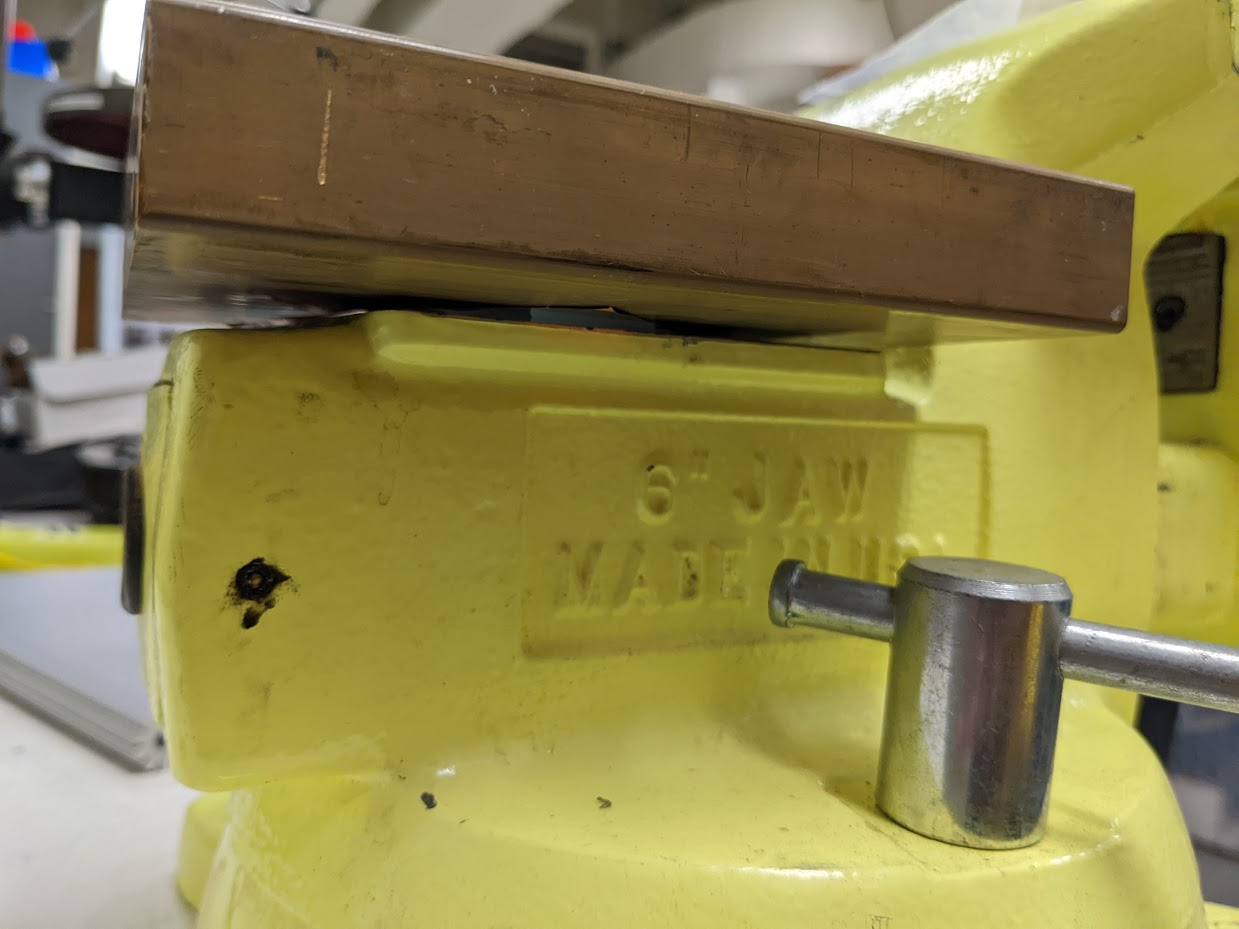
\includegraphics[width=6in]{graphics/squished_sample_PXL_20220712_025117243.jpg}
\caption{This is a bonded sample underneath the heavy brass mass. There is copper foil between the glass and metal to provide a buffer.}
\label{fig:squished_sample}
\end{center}
\end{figure}

Previous evidence suggested that heat would improve the strength of the bond. I tried heating the bonded samples many times, both without pressure {{{{fig}}}} and with a heavy brass mass on top of the sample {{{fig}}}. However, even a small amount of heat would almost immediately break even the strongest of bonds.

\begin{figure}[htbp]
\begin{center}
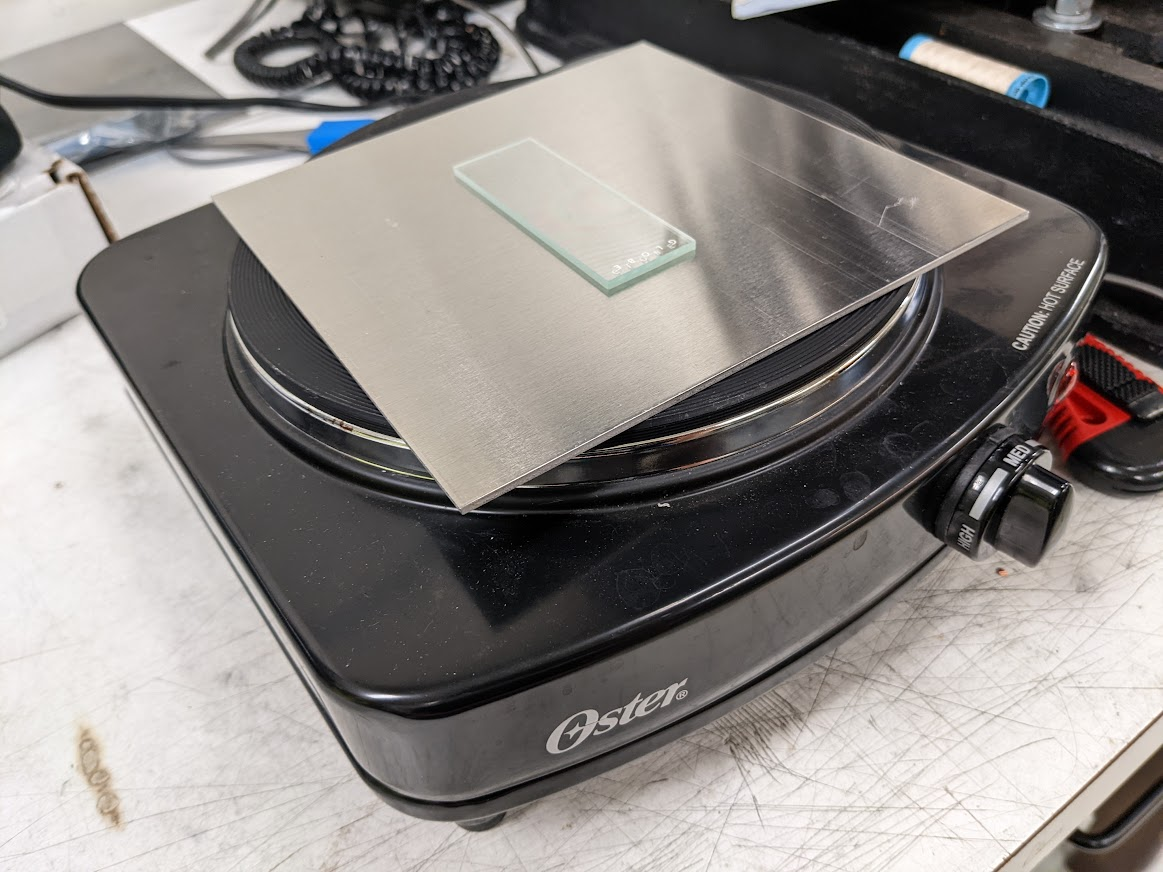
\includegraphics[width=6in]{graphics/heat_without_pressure_PXL_20220712_232551854.jpg}
\caption{To heat a sample without pressure, I simply place it on copper foil (not pictured) on the aluminum plate, which will have a thermocouple attached to it in the future, and turn on the heat. I will also sometimes preheat it.}
\label{fig:heat_without_pressure}
\end{center}
\end{figure}

\begin{figure}[htbp]
\begin{center}
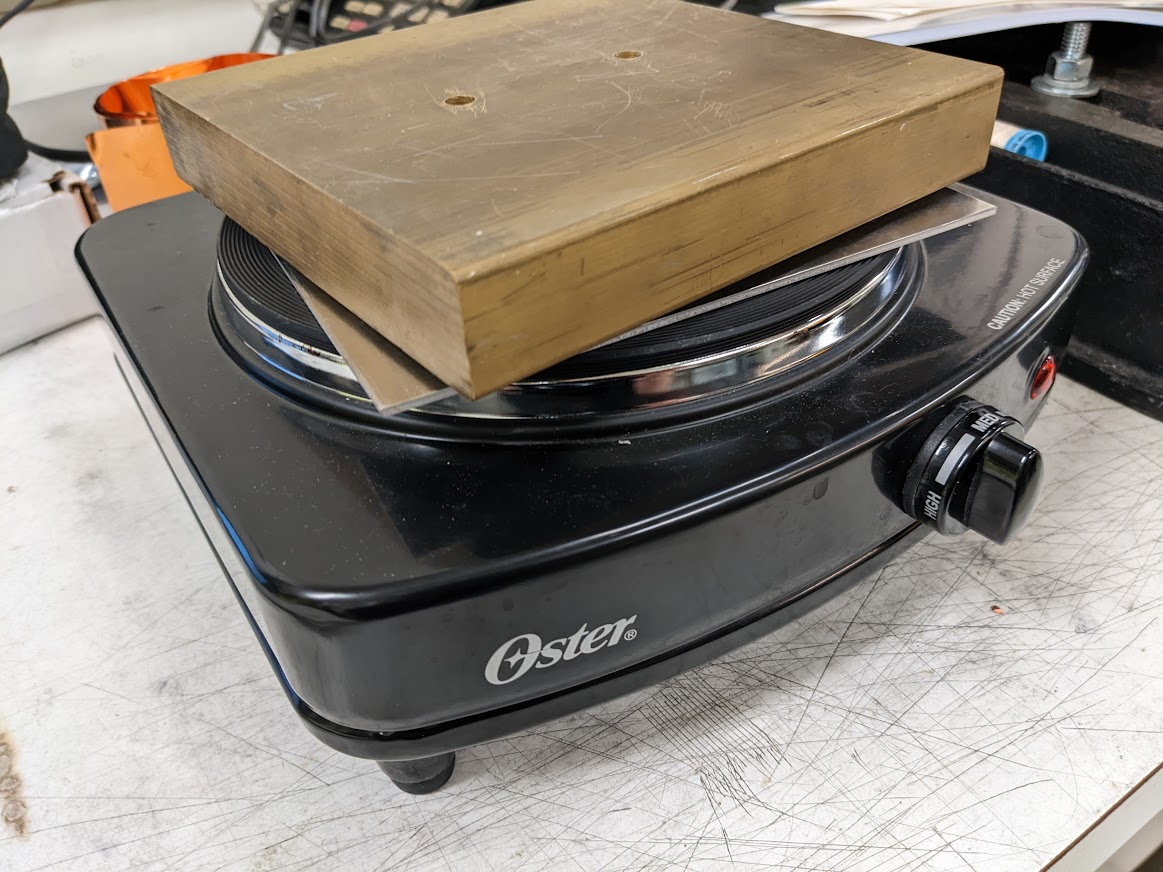
\includegraphics[width=6in]{graphics/heat_with_pressure_PXL_20220713_003923957.jpg}
\caption{To heat a sample with pressure, I do the same as without pressure, but with the brass weight on top and copper at the metal-glass interface. I cannot preheat this setup without risking burning my fingers.}
\label{fig:heat_with_pressure}
\end{center}
\end{figure}

Most recently, I have been trying to achieve a bond without the assistance of liquids, pressure, or heat. I have managed to produce a bond by scrubbing the slides with methanol, letting them dry, and then rubbing the two cleaned surfaces together while adding pressure. When I clean with methanol, I scrub with enough pressure to make them squeak. This bonding method is unreliable, and the bond is not as strong as when I use liquids.

\section{Progress}

As expected, while optical contacting seems simple on paper, actual bonding is quite difficult. I was still hoping to be a little further along by this point, but struggling with the heating conundrum and being absent from the lab slowed me down. Since I did not expect heating to break the bond, I was left a little directionless as I tried different bonding methods, mistakenly thinking that it was the method, not the heat, that was breaking the bond.

\section{Problems}

The biggest problem, as already mentioned in detail, is that the heat is unexpectedly breaking the bond instead of improving it. Although I have not identified the source of the problem, several theories have been proposed. My latest theory is that it is the rapidity of the heating that breaks the bond, but I have not been able to test it.

Another problem is that I should be able to achieve a bond without without liquid, pressure, or heat, but I have been unable to. If it is an issue of me not cleaning the glass well enough, I just need to improve my methods, like perhaps using First Contact Polymer or pressurized air during the cleaning process. If it is an issue of the glass not being polished enough, that could only be fixed by polishing the glass.

\section{Goals}

While writing this, I realized that I did not do a good job of systematically testing each method of glass bonding. I would like to spend a day or two systematically running through all the configurations of liquids (or therein lack of), heat, pressure, etc. so I have better, clearer data on what does and does not work. However, now that I have acquired silicon wafers, I would also like to start working with that as I am very curious to see if heat breaking the bond is an issue for silicon as well.

My current focus is further improving my bonding technique. If I do end up resolving the issue of heating breaking the bond, I will proceed as originally planned with creating a setup that lets me precisely control the temperature on the hot plate. Time is running short, so I am not sure if I will get to the bond quality experiments I had planned. It all depends on whether I am able to make a breakthrough on bond quality.

\begin{thebibliography}{9}
    \bibitem{Wright}
	  Wright, J. J. & Zissa,
	  \emph{D. E. OPTICAL CONTACTING FOR GRAVITY PROBE STAR TRACKER}.
	  14 (1984).    
      
    \bibitem{Rayleigh}
	  Rayleigh, Lord,
	  \emph{Optical Contact}.
	  Nature 139, 781–783 (1937).
	  
	\bibitem{Ferme}
	  Ferme, J.-J.,
	  \emph{Optical contacting}.
	  in (eds. Geyl, R., Rimmer, D. & Wang, L.) 26 (2004).
	 
    \bibitem{Zawada}
	  Zawada, A.,
	  \emph{Final Report: In-Vacuum Heat Switch}.
	  14.
    
	\bibitem{Helie}
	  Hélie, David, et al.,
	  \emph{Reinforced direct bonding of optical materials by femtosecond laser welding}.
	  Applied optics 51.12 p.2098-2106 (2012).    

	\bibitem{Ohlidal}
	  He, Mengfei, and Sidney R. Nagel,
	  \emph{Ellipsometry of layered systems}.
	  Optical Characterization of Thin Solid Films. Springer, Cham, p.233-267 (2018).

	\bibitem{Kurz}
	  Kurz, Volker Luiz Siegmar.,
	  \emph{Orientation, conformation and phase transitions of thin polymer films and self-assembled monolayers studied by SFG spectroscopy}.
	  Diss. (2010).

    \bibitem{Zawada2}
	  Zawada, A.,
	  \emph{Determining the refractive index, absolute thickness and local slope of a thin transparent film using multi-wavelength and multi-incident-angle interference}.
	  Optics Express 28.16 p.24198-24213 (2020).
  
    \bibitem{Kalkowski}
	  Kalkowski, Gerhard, et al.,
	  \emph{Glass-glass direct bonding}.
	  ECS Transactions 64.5 p.3 (2014).
 
\end{thebibliography} %Must end the environment

\end{document} 

\begin{appendices}

\section{test}

\end{appendices}